
In this section there is a more detailed overview of the platform
itself.
VLSP provides a complete environment from the
\emph{protocol stack} up to the \emph{service management} level,
including a tailor-made monitoring facility. Consequently, we are able to
experiment with new complete 5G network management and control
facilities over virtual networks based on our lightweight virtual
entity resembling both servers and routers.

 VLSP is a distributed management
infrastructure that has centralized functionality and is
responsible for the setup, configuration, optimization, and shutdown
of network entities.
 It has been implemented for the
purpose of testing and evaluating various aspects of managing  highly dynamic virtual
environments, in particular  the 6 aspects of:

\begin{adjustwidth}{\parindent}{}
\begin{enumerate}[label=(\roman*),noitemsep]
\item efficient service function,
\item optimized service function availability,
\item service and VNF lifecycle automation,
\item service placement automation,
\item efficient resource utilization, and
\item  dynamic resource up/down scaling (elasticity).
\end{enumerate}
\end{adjustwidth}

\noindent VLSP is a testbed that consists of a large number of virtualized entities which
execute on a number of physical machines.
The entities are logically independent software entities that
communicate with each other via network interfaces. 
The testbed has been validated
for some of these aspects in previous work we have undertaken on
virtualized and highly dynamic networks.

The VLSP set up has various components described in this section
and include:

\begin{adjustwidth}{\parindent}{}
\begin{enumerate}[label=(\roman*),noitemsep]
\item a supervisor and experimental
controller realizing the basic functionalities of an Orchestration
Layer  / Virtual Infrastructure Management (VIM) called the  \textit{Global Controller};

\item per-host \emph{Host Controllers};  and

\item the \emph{virtualized entities}, which run inside a JVM.
\end{enumerate}
\end{adjustwidth}

\noindent VLSP is configured by the \emph{Global Controller} running 
on one physical server, and the \emph{Host Controllers} running on
physical machines that host virtual entities.
Under control of the
\emph{Global Controller}, the individual \emph{Host Controllers}
start or interact with virtual entities when needed. The choice of
\emph{Host Controller} is decided by the \emph{Placement Engine},
which uses an algorithm to determine the \emph{best} physical machine
to deploy the new virtual entity.  The \emph{Global Controller} also
sends requests, via a \emph{Host Controller}, to 
connect virtual routers together via virtual  links.

In order to manage the challenging and dynamic infrastructures of
virtual networks there needs to be a monitoring system which collects
data and reports on the behavior of both the physical resources
(e.g. CPU usage, memory usage) and the virtual resources
(e.g. utilization level of the virtual links). The monitoring data
items are sent to the \textit{Global Controller} components. The
monitoring information is used to take decisions regarding network
strategies and enforces these decisions. The monitoring system
\emph{Lattice} is used as has been proven to be ideal for the task of
collecting monitoring data for various types of dynamic network
environments.  Each virtual entity has at least one probe that can
generate data. Monitoring data is also collected from each \emph{Host
  Controller}. All of this monitoring data is send to the \emph{Global
  Controller}, and it is the data that is used by the \emph{Placement
  Engine} for determining where a new virtual entity is placed.


\subsection{Main Function Elements}



The main elements of the Platform are the Orchestration
Layer  / Virtual Infrastructure Management (VIM) called the  \emph{GlobalController},
the per-host \emph{Host Controllers}, called the \emph{LocalControllers}, and the \emph{Routers}.  These are each
explained in further detail below.

The main elements can be found in the following table.

\begin{longtable}{ | p{5cm} | p{9cm} | }

\hline
\textbf{Name} & \textbf{Description} \\
\hline
Host Controllers & The host controllers execute on every physical
machine and manipulate and configure virtual routers, links and virtual
router applications. \\
\hline
Monitoring System & The monitoring system, comprising probes that are tiny configurable applications
probing the software or hardware for monitoring data, as well as the
data consumers. \\
\hline
Event Management & It is responsible for the runtime operation,
including support for event-based notifications and time scheduling. \\
\hline
Virtual Router Protocol Stack & The lightweight network protocol stack
of the VRs.  \\
\hline
Virtual Router Application Environment & The application environment that hosts VR applications. \\
\hline
Virtual Link Functionality & The functionality of the virtual links,
including link weighting and other configuration options. \\
\hline
Virtual Machine for Virtual Router and Application Functionality & A
virtual machine with the virtual router and the relevant applications
functionality. \\
\hline

\end{longtable}

\noindent There is one \emph{VIM} for the platform, and it has the
following functions:

\begin{itemize}
\item it starts and stops the LocalControllers
\item it acts as a control point for the platform by sending out commands, 
\item it acts as a management element for the platform by collecting
  monitoring data and enabling reactive behaviour 
\end{itemize}

\noindent The Virtual Infrastructure Management (VIM)  can run on the same host as a
LocalController, or in a large setup it can run on a separate host.
The VIM component is responsible
for the management and lifecycle of the virtualized elements that will
be used within a network, particularly virtual network elements. As
the virtual elements are not physical themselves, but exist on top of
physical elements, their lifecycle and their management needs to be
approached carefully to ensure continued operation and consistency.

The virtual network elements, which exist on top of physical networks,
can be setup with arbitrary topologies and with an arbitrary number of
end-points. The virtual links in a virtual topology are eventually
mapped onto physical links in the underlying network. A virtual link
may span multiple physical links, and cross many physical routers, or
it may span a single physical network link. New virtual links can be
added or can be removed from a virtual network dynamically at
run-time.

The virtual networks are very flexible and adaptable, and generally
have few limitations, except that a virtual link cannot support more
traffic and higher-data rates than the underlying physical
links. Furthermore, a whole virtual network can be shutdown as needed,
if the applications that use it no longer need the network. Such a
shutdown frees resources from the underlying physical network.

%% The full management of virtual networks on physical networks requires
%% the matching and analysis of the flow rates on the virtual links to
%% the flow rates of the underlying physical links. It is important to
%% ensure that the physical links are not congested with too many virtual
%% links. Also, the allocation and mapping of virtual links must take
%% into account the current state of the physical network and the current
%% virtual networks. However, if a situation arises where a
%% re-configuration is required, the virtual network management should be
%% capable of mapping a virtual link across different physical links at
%% run-time, but leave the virtual topology intact.

The VIM component has a seemingly simple task, but in reality the
management requires continual monitoring, analysis, and adaption of
the virtual elements to the physical elements. As all of these virtual
elements are distributed, the management is a complex task.
The VIM interacts with the virtual network
elements that will be present in a running virtual network. All of the
elements of the VIM component constitute a fully distributed system,
whereby an element or node can reside on any host. A full virtual
network can be instantiated on a single machine, for demonstration or
testing purposes, or instantiated across multiple servers, in a full
deployment situation.

The VIM directly controls the lifecycle of each virtual element, by
collecting knowledge on the status of physical resources in order to
determine where a virtual element can be created. The virtual network
element will be created, managed, and shutdown by lifecycle phase of
this component.

Due to the dynamic nature of virtual elements and because they can be
disassociated from the physical elements they are mapped to, it is
possible to do a live adaption of a virtual element from one physical
host to another physical one, at run-time.

The VIM controller acts as a control point for managing the virtual
elements. This block accepts all its input via the VIM REST interface
from other management applications / network services. The monitoring
engine acts a collection point for the monitoring data needed to keep
the management functions running. Control commands are sent to
the VIM and they are either acted upon immediately or are passed to
the corresponding Host Controllers.

The main VIM elements can be found in the following table.
\begin{longtable}{ | p{5cm} | p{9cm} | }

\hline
\textbf{Name} & \textbf{Description} \\
\hline
VIM Controller & It is the heart of the component, providing the
central control of the VIM operations. \\
\hline
Scripting Engine & VIM can be configured using Closure
scripting. \\
\hline
Monitoring Engine & It is the main monitoring component of the
infrastructure, i.e., collecting \& manipulating measurements from the
monitoring probes residing at the virtual entities. \\
\hline
Virtual Entities / Topology Configurators & These functions are responsible for the configuration of virtual routers, links and topologies, supporting different levels of abstraction. \\
\hline
Configuration Actuators	& The Virtual Entities / Topology
configurators communicate with the configuration actuators which in
turn enforce the configuration changes through the LNH's host
controllers. \\
\hline
\end{longtable}


There is one \emph{LocalController} for each physical host that needs
to execute virtual routers.  A LocalController has the following
functions:

\begin{itemize}
\item it starts and stops virtual routers
\item it tells routers to create and remove virtaul network
  connections
\item to get or set attributes on routers or links
\end{itemize}

\noindent A LocalController is similar to a hypervisor in a normal
virtualization environment, as it has a role of stopping and stopping
virtaul machines.

Within the platform, many \emph{Routers} can be created.  These
virtaul routers behave like a real hardware router, with the caveat
that they have much simpler functionality.

\begin{figure}
    \centering
    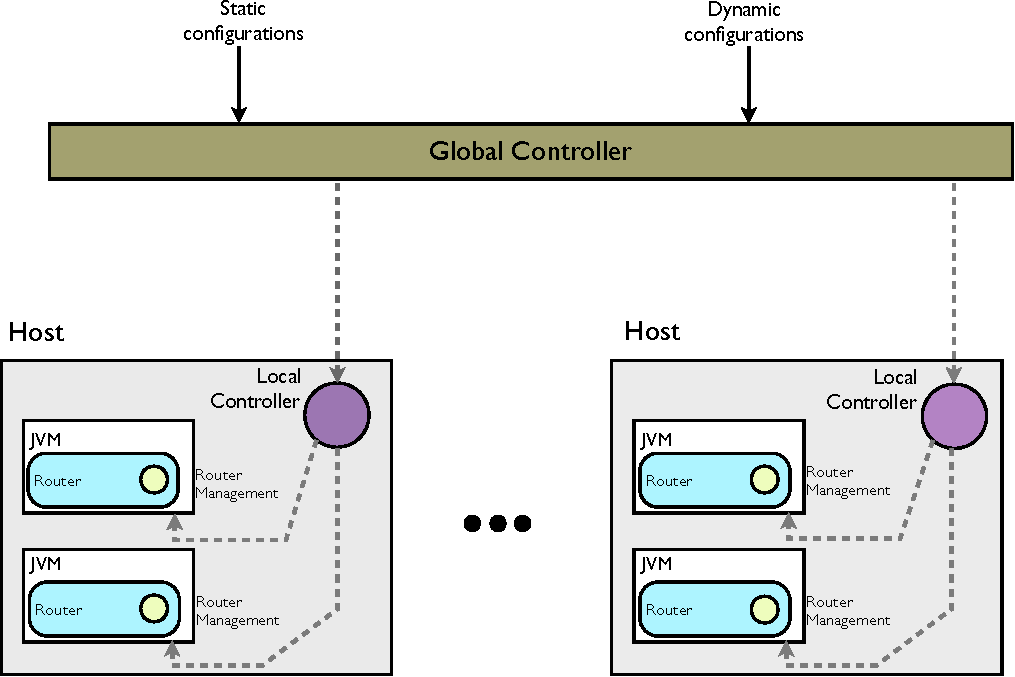
\includegraphics[width=13cm]{images/architecture}
    \caption{General Architecture}
    \label{usr-architecture}
\end{figure}

In figure \ref{usr-architecture}, the relationship between these
elements is shown. There is the VIM / GlobalController, shown in brown, which can take
various configurations in order to setup and control a run.  These
configurations can be static configurations, where there is a fixed
topology, or dynamic configurations, where the topology of the network
and the number of links changes on-the-fly under the control of the
GlobalController.

The GlobalController interacts with various LocalControllers.  This
interaction path is shown as a dotted line.  A LocalController,
shown in purple,
executes on each physical host that participates in the platform.
Each LocalController takes requests from the GlobalController and
takes the required action.  This can be to start or stop a virtual
router, to create or remove a virtual link, to get or set attributes
on routers or links.

To start a new Router, shown in blue, the LocalController on the
relevant host will start a new Java Virtual Machine, shown in white,
executing the specific Router code.  The router has various elements,
which will be discussed later, however for this discussion the most
important one is the Router Management element, shown in yellow.  Once
a Router is up and running, the LocalController interacts with it via
the Router Management interface.  It is using this interface that
commands and requests for the Router are sent by the
LocalController. This path is also shown via a dotted line.


Although there is a considerable amoount of infrastructure in the
platform dealing with control, the main aim of the platform is to
create a topology of virtual 
routers.  These routers execute on a set of hosts, with virtual links
between the virtual routers. 
In figure \ref{usr-hosts}, we see how the topology of virtual routers
and virtual links manifests itself across multiple hosts, three in this
case. 

\begin{figure}[h!]
    \centering
    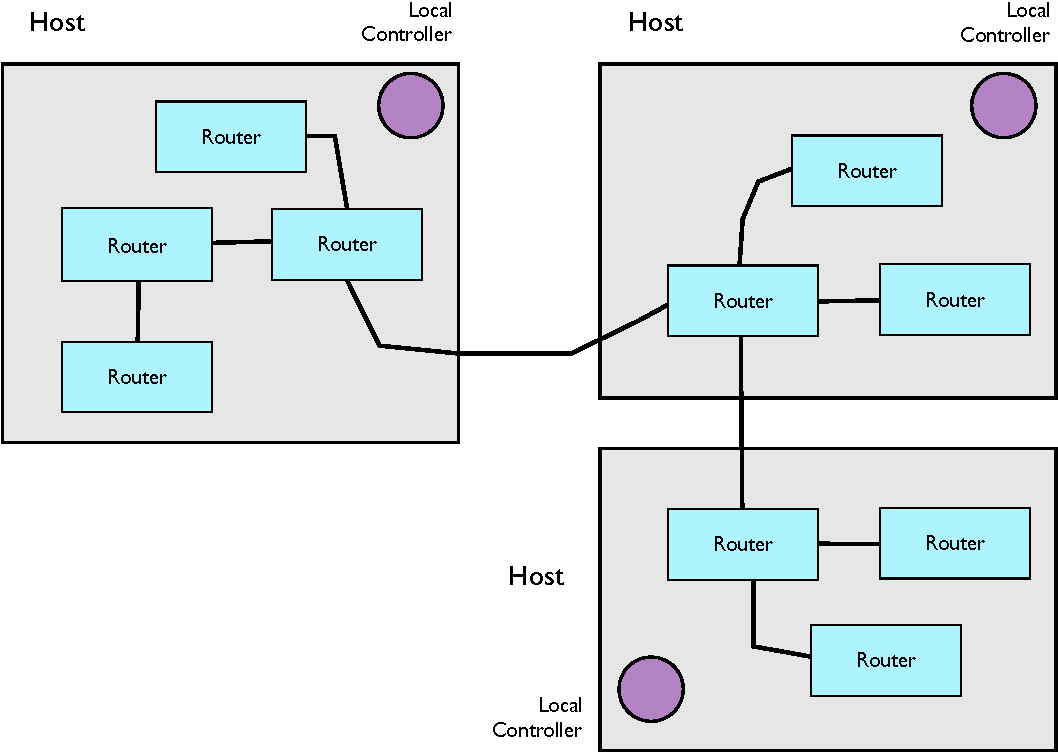
\includegraphics[width=13cm]{images/hosts}
    \caption{Hosts with Virtual Routers and Virtual Links}
    \label{usr-hosts}
\end{figure}

An alternative view of the platform where the hosts are not shown, but
there is the control path and the virtual routers and virtual links is
shown in figure \ref{usr-control}.
Control propogates from the GlobalController, via the
LocalControllers, to the Routers.
The topology of Routers is connected by separate virtual links.

\begin{figure}[h!]
    \centering
    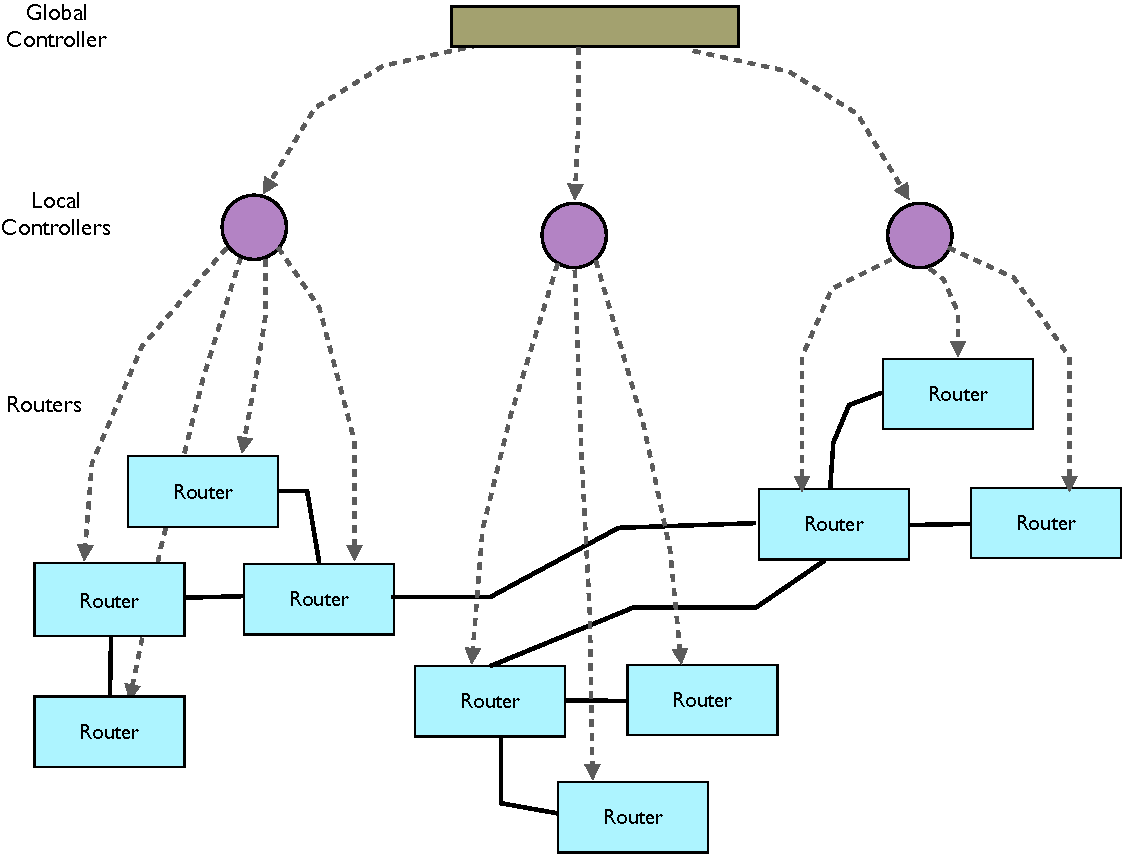
\includegraphics[width=13cm]{images/control-path}
    \caption{Full Connectivity with Control Path}
    \label{usr-control}
\end{figure}


\subsection{Main Platform Functions}

The main functions of the  Very Lightweight Network \& Service
Platform are outlined in this subsection. 
The platform uses a set of Virtual Routers and Virtual
Network Connections to create a test environment which can easily
accommodate:
\begin{itemize}
\item fast setup / teardown of a Virtual Router
\item fast setup / teardown of a Virtual Connection
\item each Virtual Router can run small programs / service elements
\end{itemize}

\noindent These are explained in more detail in the following sections.

\subsection{Routers}

The software virtual router is implemented in Java and is a relatively complex 
software entity.  The routers hold network selections to the other virtual
routers they are aware of and exchange routing tables to determine the 
shortest path to each other router.  Datagrams are sent between routers
and queued at input and output.  A system of virtual ports (like the 
current transport layer ports) are exposed with an interface very similar
to standard ``sockets".  Virtual services can be run on the virtual
routers and listen and send on the virtual sockets. 
The datagrams themselves, have headers 
with a source address, destination address, protocol, source port, destination port,
length, checksum and time to live -- many of the features of real UDP
packets are replicated.  

\subsection{Routing and packet transmission}

Routing in these virtual routers is distance-vector based.  To prevent routing storms
minimum times between table transmissions are set.  In addition, because
the experiment here demands a certain ``churn" of virtual routers
then addresses which disappear permanently must be dealt with.  In distance
vector routing it is well-known that dead addresses can leave routing loops.
This is dealt with in the current system by implementing time to live
(TTL) in packets and
also implementing a maximum routing distance beyond which a router is assumed
unreachable and removed from routing tables.

Virtual services can run on the routers.  Naturally the only important
virtual services for the purposes of our evaluations are networked
services.  The services
tested include simple network test protocols such as ping and traceroute and
ftp style send and receive services.
The major software used, however, is the Lattice monitoring framework developed for
 RESERVOIR.  
The virtual services can listen on virtual ports and send datagrams to any
address and virtual port.

Datagrams are queued both inbound and outbound, the outbound queue is blocking 
in order that transmitting services can slow their sending rate.
The inbound queue is tail-drop so that when too much traffic is sent drops
will occur somewhere.  TTL is decreased at each hop and, on expiry, a "TTL
expired" packet is returned -- this allows the virtual router system to
implement traceroute as a virtual service.  Virtual routers in the 
system send all traffic including routing tables and other control messages
via network sockets.  Control messages (routing tables, echo, echo reply,
TTL expired and so on) are routed in the same way as data packets on a
hop by hop basis using the routing tables.  
Datagram transmission is UDP-like in this
iteration of the system, that is, delivery is not guaranteed and a failure
to deliver will not be reported to the service (although if the router
on which a virtual service runs
has no route to the host this can be reported to the service).

\subsection{Start up and tear down}

Start up and tear down for routers is scheduled by the Global Controller
and directly performed by the Local Controller which resides on each
physical machine as the virtual router.   The
virtual routers would operate perfectly well without such a controller,
for example, if they were set up and connected manually or by some other
distributed control system.  The Local Controller is necessary to
spawn off new routers on a machine.
In addition, the Local Controller is used here to
pass on Global Controller commands to shut down or connect virtual
routers.  

\subsection{Virtual Services / Applications}

Each virtual router has a socket interface by which services and
applications can be written.  All networking interactions are done using
our USR Datagram layer, which is very similar to the standard Java
socket and datagram interface.
Each service can open a socket on a given address and port, and
can send traffic to an address and a port.

By having our own virtual datagram layer we could control all the
networking within the virtual router.  However, by making the socket
and datagram interface very similar to the standard Java one, we were
able to utilize existing Java software which has a standard UDP
mechanism.

As an example of easy re-used of existing software, consider that it
took just a few hours to port the Lattice monitoring
framework onto this new platform.  We wrote an implementation of the
data plane using USR instead of UDP.  In terms of the source code,
there are few differences between each implementation.

\subsection{Monitoring}

The monitoring software used in VLSP is called Lattice and has been
used for monitoring virtualised services in federated cloud
environments, for monitoring virtual networks, and as the
monitoring system for an information management platform that
aggregates, filters, and collects data in a scalable manner within
virtual networks. Lattice, which is also an open-source
software, has been proven to be ideal for the task of collecting
monitoring data for various types of dynamic network environments.

Each virtual router has a set of probes which generate data for
virtual link usage, cpu / memory usage per thread, and virtual
applications resource consumption. This data is sent to the Monitoring
Engine of the Global Controller which processes it. This data is
used by the Placement Engine for determining where a new virtual
router is placed. 

\subsection{REST API for Dynamic Programmable Control}

A dynamic programmable control environment allows the definition of
scenarios, resources, or other software entity parameters using
appropriate functions via a REST API. In our case, we use a Java
client or one written in the Clojure language
for the dynamic configurations. This allows us to perform fully
Software-Defined Operations using a functional language that has an
expressive representation of the configuration settings, while being
very brief.

\subsection{Event Engine for Probabilistic Experiment Control}

Many experiments that are undertaken in the networking domain are
based on arrival rates that are taken from a probability
distribution. Within VLSP we have an \emph{event engine} that can generate
events to create a router, destroy a router, create a link, and delete
a link, all based on probability distributions.

For any particular run
we can specify these distributions together with their associated
parameters in an XML configuration file. The options for the
distribution are set 
in a Type field as one of: Uniform, Exponential, LogNormal, or
PoissonPlus, matching well-known topology models. Fur- thermore, we
are providing pre-defined configuration files with realistic
topologies, e.g. for data centers. 

\subsection{VLSP Visualization}

One of the management tools we have built for VLSP is a Network
Visualization tool. It takes a logical graph view of the virtual
topology, including the routers and the links, and presents a
visualization graph by using the graphviz tool. From data held by the
Orchestration Controller, a version of the network is generated in the
dot language that graphviz uses. As dot is very flexibile, it is easy
to create extensions to the visualizations which include the virtual
applications that execute on the routers. Furthermore, we are able to
present key nodes in different shapes and colours in order to
highlight the different features of a topology. As an example,
consider the topology on the cover which represents a partial snapshot
from one of our experiments. Those with a similar colour are 
logically connected for managing the same data streams, and those
nodes represented as a diamond shape are running a Data Proxy
application. It allows us to see how data management applications are
deployed across the whole topology. 
